\chapter{Image Denoising}

\section{Thermal noise}
\begin{itemize}
\item Significative in \gls{MRI}.
\item Originated by the thermal motion of the atoms and therefore, of
  the electrons.
\item Described as a grainy, random texture.
\item Modeled as additive Gaussian noise or, in the case of \gls{MRI}
  as additive Rician noise, because the noise is captured in the
  frequency domain.
\end{itemize}

\section{Quantum mottle (quantum noise)}
\begin{itemize}
\item Appears in X-ray and \gls{CT} images.
\item Consequence of the \popup{small number
    of photons}{Remember that the radiation must be minimized and the
    number of X-ray photons is proportional to the energy of the
    radiation.} that reach the detector.
\item Looks like grainy noise. 
\item Mathematically modeled as a \popup{(multiplicative)}{By
    definition, Poisson noise is multiplicative.} Poisson
  distribution.
\end{itemize}

\section{Speckle (interference) noise}
\begin{itemize}
\item Significative in low-SNR areas of \gls{MRI} images and in ultrasound images.
\item Generated by the constructive and destructive interference of
  \popup{coherent waves}{Waves are in phase.}, such as laser light or
  radar waves, interacting with a target.
\item Described as granular, textured pattern.
\item Usually modeled as multiplicative Gamma distribution (or more
  specifically, a Rayleigh distribution for the signal amplitude).
\end{itemize}

\section{Physiological noise}
\begin{itemize}
\item Significative in \gls{MRI}, and it is independent of $B_0$ (the
  strength of the magnetic field).
\item Refers to undesired signal variations caused by the patient's
  own bodily functions, primarily cardiac (heartbeat) and respiratory
  (breathing) cycles. These processes induce changes in cerebral blood
  flow, blood volume, and cerebrospinal fluid flow, generating
  magnetic field fluctuations.
\item Non uniform (depends on the scanned area) and difficult to model.
\end{itemize}

\section{Denoising}
\begin{itemize}
\item Denoising (the removal of the noise) is carried out in
  medical imaging to improve the \gls{SNR}, with the ultimate
  objective of increase the accuracy of the diagnoses.
\item Unfortunately, it is difficult to remove only noise (some part
  of the signal, typically the high frequency components of the signal
  are also filtered-out.
\end{itemize}

\section{Gaussian filtering}
\begin{itemize}
\item Spatial (2D) filter \popup{using 1D Gaussian}{The filter is
    separable, which means that the image can be filtered by rows and
    columns, using always 1D kernels.} \popup{kernels}{Filter is
    another name for the filter structure.}.
\end{itemize}
\vspace{-4ex}
\begin{center}
  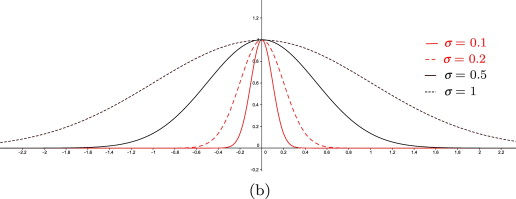
\includegraphics[width=6cm]{Gaussian_kernels}
\end{center}
\vspace{-4ex}
\begin{itemize}
\item Isotropic (it \popup{blurs pixel values equally in all directions}{Which
    softens noise but also destroys important edges.}).
\end{itemize}
\begin{center}
    \href{https://www.cloudfactory.com/blog/gaussian-noise-medical-ai}{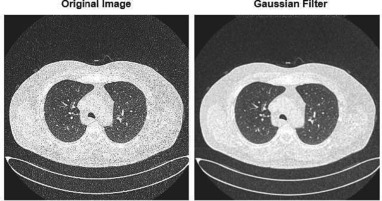
\includegraphics[width=\textwidth]{GF_example}}
\end{center}

\section{Anisotropic diffusion filtering}
\begin{itemize}
\item Anisotropic (only blurs in the direction of the minimum
  gradient, i.e., the edged are preserved).
\end{itemize}
\begin{center}
  \href{https://dsp.stackexchange.com/questions/14606/anisotropic-diffusion}{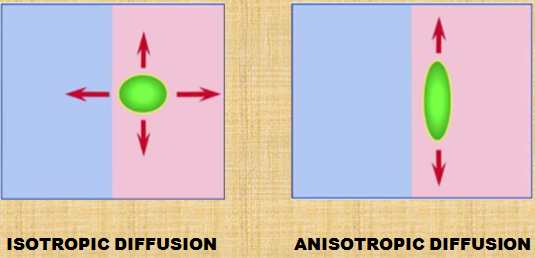
\includegraphics[width=8cm]{anisotropic_diffusion}}\\
  (The kernel is longer in the direction of the edge.)
\end{center}
\begin{center}
    \href{https://es.mathworks.com/help/images/ref/imdiffusefilt.html}{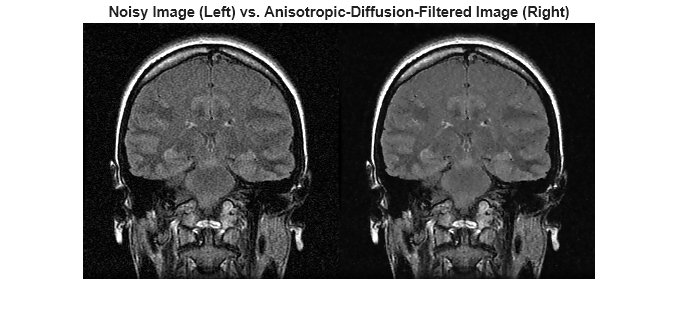
\includegraphics[width=\textwidth]{AD_example}}
\end{center}

\section{Wiener denoising}
% Include also filtering in the wavelet domain because can be useful for removing specke noise.
\vbox{
\begin{itemize}
\item Wiener developed an adaptive filter based on a predictor capable
  of restore the \popup{image}{A signal in general.} in several
  aspects, for example,
  \href{https://docs.opencv.org/3.4/d1/dfd/tutorial_motion_deblur_filter.html}{to
    correct the blur generated by motion}.
\begin{center}
  \href{https://docs.opencv.org/3.4/white_car.jpg}{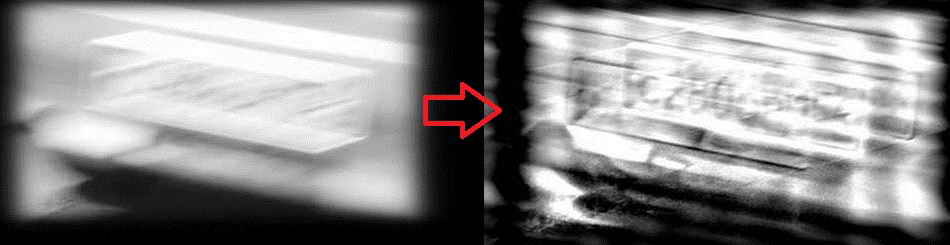
\includegraphics[width=12cm]{wiener_deconvolution}}\\
  (Motion de-blur using Wiener deconvolution.)
\end{center}
\end{itemize}
}
\vbox{
\begin{itemize}
\item Using a Wiener filter we can also \popup{remove}{The correct
    word here (and in all the denoising techniques) should be
    ``minimize''. Only if the noise signal were known, the original
    (clean) signal could be completely restored.}  \popup{additive
    noise}{A random signal that has been added to the clean signal,
    and that is independent of the clean signal.} of a image by
  estimating the amplitude of the noise. The idea is to use a
  \popup{bluring filter}{A low-pass filter, such as a Gaussian kernel}
  \popup{adapted to the energy of the noise}{The higher the amplitude
    of the noise, the longer the kernel, i.e., the higher the blur
    effect, and therefore, the higher the noise removal.} \popup{in
    each area}{For this reason, one of the parameters of the Wiener
    filter for denoising is the size of a square window.} of the
  image.
\end{itemize}
\vspace{-4ex}
\begin{center}
  \href{https://www.techscience.com/csse/v45n2/50440/html}{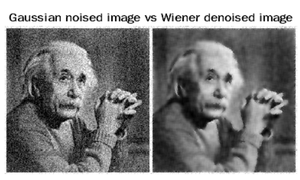
\includegraphics[width=10cm]{wiener_albert}}\\
  (Removal of Gaussian noise using Wiener denoising.)
\end{center}
}

\section{\gls{NLM}}
\vbox{
  \begin{itemize}
  \item Most images are redundant in terms of the different local
    textures and patterns that define them.
    \begin{center}
      \href{https://docs.opencv.org/3.4/d5/d69/tutorial_py_non_local_means.html}{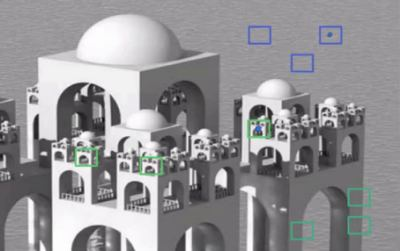
\includegraphics[width=8cm]{NLM_opencv}}\\
      (Patch averaging.)
    \end{center}
  \end{itemize}
}
\vbox{
  \begin{itemize}
  \item The mean of the noise \popup{is usually zero}{And if the mean
      ins not zero, we can substract the mean of the noise.}, i.e.,
    the average of different instances of the same signal tends to the
    clean signal logarithmically.
    \begin{center}
      \href{https://www.umbjournal.org/article/S0301-5629(17)30201-6/fulltext}{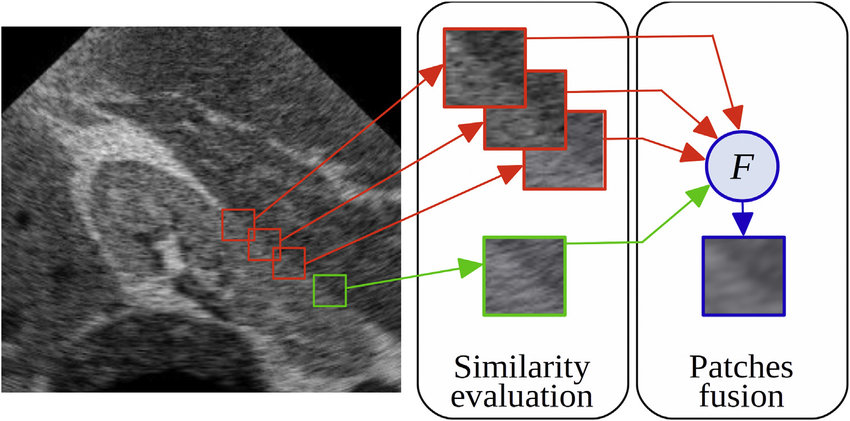
\includegraphics[width=10cm]{NLM_example}}\\
      (Patch averaging.)
    \end{center}
  \end{itemize}
}
\vbox{
  \begin{itemize}
  \item An \gls{NLM} denoising
    \href{https://imagej.net/plugins/non-local-means-denoise/}{example}:
    \begin{center}
      \begin{tabular}{cc}
        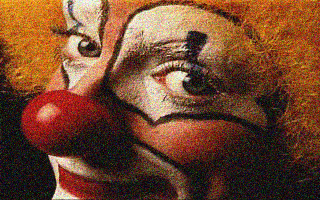
\includegraphics[width=6cm]{clown-noise-25} & 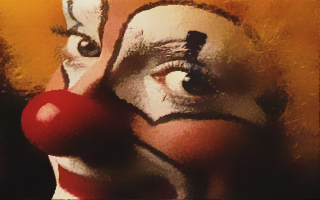
\includegraphics[width=6cm]{NLM_clown}
      \end{tabular}
    \end{center}
  \end{itemize}
}

\section{\gls{AI}-based denoising}
\vbox{
  \begin{itemize}
  \item \gls{AI} denoisers are adaptive filters that learn by
    (thousands of) example(s). In each iteration, at the input you put
    a noisy image and at the output a noise-free version of such
    image.
  \item Most of them are based in \glspl{CNN}. A \gls{CNN} is a
    \popup{feed-forward}{The data flows fron the input to the output
      without loops.} \gls{ANN} in which the
    \popup{neurons}{Convolutional.} (that are organized in
    \popup{layers}{Convolutional.}) have a local (spatial)
    relationship with the neurons of the next layer.
    \begin{center}
      \href{https://en.wikipedia.org/wiki/Convolutional_neural_network#/media/File:1D_Convolutional_Neural_Network_feed_forward_example.png}{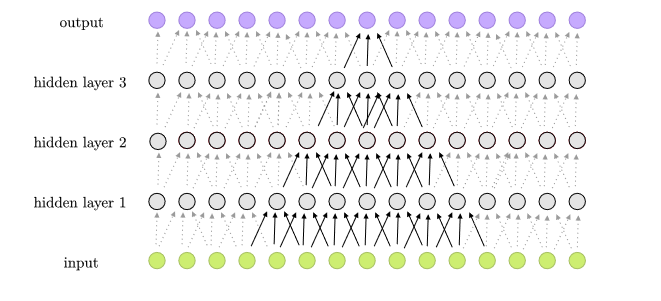
\includegraphics[width=8cm]{1D_Convolutional_Neural_Network_feed_forward_example}}\\
      (A 1D \gls{CNN} where the connection degree (kernel size) is 3.)
    \end{center}
  \end{itemize}
}

\vbox{
  \begin{itemize}
  \item Using
    \href{https://en.wikipedia.org/wiki/Backpropagation}{back-propagation}
    the neurons learn which must be the weights between them to
    minimize the \popup{error}{Some definition of the error, for
      example, the MSE.} between the input and the output.
  \item There can be several \popup{channels}{In the previous example
      there is only one channel per layer.} per layer.
  \item A feature map is the array with the output of each neuron in a
    channel.
    \begin{center}
      \href{}{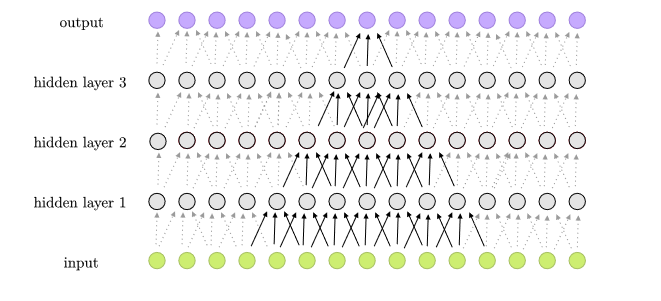
\includegraphics[width=8cm]{1D_Convolutional_Neural_Network_feed_forward_example}}\\
      (A 1D \gls{CNN} where the connection degree (kernel size) is 3.)
    \end{center}
  \end{itemize}
}

\vbox{
  \begin{itemize}
  \item When the number of neurons per layer decreases from the input to the output.
    \begin{center}
      \href{}{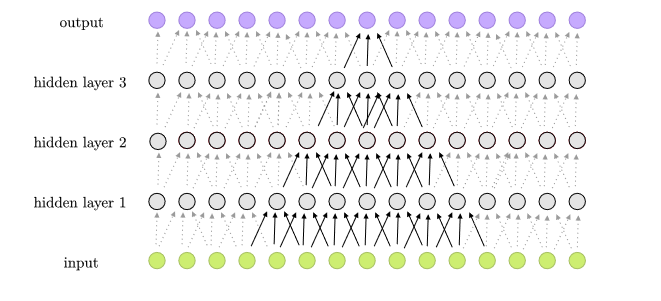
\includegraphics[width=8cm]{1D_Convolutional_Neural_Network_feed_forward_example}}\\
      (A 1D \gls{CNN} where the connection degree (kernel size) is 3.)
    \end{center}
  \end{itemize}
}

How They Work

Contracting
path (left side) and an expansive path (right side

Unlike traditional methods that rely on fixed mathematical algorithms (like Gaussian filters or wavelet transforms), deep learning models learn how to denoise.

The typical process involves training a neural network on a massive dataset of paired data:

    Clean Data: The original, noise-free image or signal.

    Noisy Data: The same data with noise artificially added.

    The network's goal is to learn the complex mapping required to transform any noisy input back into its clean, original state. By doing this, it learns the underlying structure of the signal and can distinguish it from the characteristics of the noise.

Key Architectures Used

Several types of neural networks are particularly effective for this task:

    Denoising Autoencoders: A classic approach where a network learns to compress a noisy image into a compact representation (encoding) and then reconstruct a clean version from it (decoding).

Convolutional Neural Networks (CNNs): The most popular and powerful method for image denoising. Architectures like DnCNN (Denoising CNN) and U-Net are specifically designed to process images, effectively learning to identify and remove noise while preserving important details like edges and textures.

Generative Adversarial Networks (GANs): These models use a "generator" network to create clean images and a "discriminator" network to distinguish them from real clean images. This adversarial process pushes the generator to produce extremely realistic, high-quality denoised results.

AI vs. Traditional Denoising

Feature	Traditional Denoising	AI-Based Denoising
Principle	Relies on fixed mathematical models (e.g., averaging, transforms).	Learns from data to distinguish signal from noise.
Adaptability	Not very adaptable; optimized for specific noise types.	Highly adaptable; can handle complex and mixed noise.
Data	Requires no training data.	Requires a large dataset of noisy/clean pairs for training.
Performance	Can cause blurring and loss of fine details.	Excels at preserving details and texture, often achieving superior results.

Singh, P. (2025). Understanding Medical Image Denoising, Enhancement, and Reconstruction. Biomedical Informatics and Smart Healthcare, 1(1), 35–39. https://doi.org/10.62762/BISH.2025.966762

Gaussian,  or non-local means